\documentclass[twocolumn,10pt]{article}
\usepackage[utf8]{inputenc}
\usepackage[margin=0.75in]{geometry}
\usepackage{amsmath,amssymb}
\usepackage{chemfig}
\usepackage{chemformula}
\usepackage{tikz}
\usepackage{enumitem}
\usepackage{titlesec}

\title{2023 U.S. National Chemistry Olympiad\\National Exam Part I}
\date{}
\author{}

\begin{document}

\maketitle

\section*{DIRECTIONS}
When you have selected your answer to each question, blacken the corresponding space on the answer sheet using a soft, \#2 pencil. Make a heavy, full mark, but no stray marks. If you decide to change an answer, erase the unwanted mark very carefully. There is only one correct answer to each question. Any questions for which more than one response has been blackened will not be counted. Your score is based solely on the number of questions you answer correctly. It is to your advantage to answer every question.

\begin{enumerate}[label=\arabic*., leftmargin=*]

\item An amino acid ($M=174$) with a formula of \ch{C_a H_b N_x O_2} contains 8.1\% by mass of H and 41.3\% by mass of C. What is the value of $x$ in its formula?
\begin{enumerate}[label=(\Alph*)]
    \item 1 \item 2 \item 3 \item 4
\end{enumerate}

\item Potassium tris(oxalato)ferrate(III) trihydrate is prepared by precipitation from aqueous solution according to the following equation:
\[ 3\,\ch{K2C2O4}(aq) + \ch{FeCl3}(aq) + 3\,\ch{H2O}(l) \rightarrow \ch{K3Fe(C2O4)3.3H2O}(s) + 3\,\ch{KCl}(aq) \]
A student mixes 10.00~g \ch{K2C2O4} ($M=166.2$) and 5.00~g \ch{FeCl3} ($M=162.2$) in 20.0~mL water and isolates 5.74~g \ch{K3Fe(C2O4)3.3H2O} by filtration. What is the percent yield of this reaction?
\begin{enumerate}[label=(\Alph*)]
    \item 19.4\% \item 37.9\% \item 58.3\% \item 65.5\%
\end{enumerate}

\item Carbon tetrachloride (\ch{CCl4}, $M=153.8$, $\text{density} = 1.59\text{ g mL}^{-1}$) and heptane (\ch{C7H16}, $M=100.2$, $\text{density} = 0.68\text{ g mL}^{-1}$) are miscible liquids. Which solution has the highest concentration of \ch{CCl4}?
\begin{enumerate}[label=(\Alph*)]
    \item 5\% v/v \ch{CCl4} in heptane
    \item 5\% w/w \ch{CCl4} in heptane
    \item 5 mol\% \ch{CCl4} in heptane
    \item All three solutions have the same concentration of \ch{CCl4}
\end{enumerate}

\item A solution of 5.00~g of which substance dissolved in 100.0~g water has the highest boiling point?
\begin{enumerate}[label=(\Alph*)]
    \item \ch{H3PO4} \item \ch{H2SO4} \item \ch{H3AsO4} \item \ch{H2SeO4}
\end{enumerate}

\item A 1.802-g sample of a hydrated double salt containing two different metal ions with the formula of $\ch{M_A(M_B)2(SO4)4.22H2O}$ is heated strongly to drive off all the water, leaving a residue of 1.000~g. What is the identity of $\ch{M_A}$?
\begin{enumerate}[label=(\Alph*)]
    \item \ch{Ca^{2+}} \item \ch{Ti^{4+}} \item \ch{Fe^{2+}} \item \ch{Ba^{2+}}
\end{enumerate}

\item Hypochlorite ion reacts with hydrogen peroxide to produce oxygen gas:
\[ \ch{OCl-}(aq) + \ch{H2O2}(aq) \rightarrow \ch{H2O}(l) + \ch{Cl-}(aq) + \ch{O2}(g) \]
A series of experiments is carried out where 10.0~mL of a 0.30~M solution of hydrogen peroxide is mixed with a varying volume of 0.40~M sodium hypochlorite solution, and the oxygen gas evolved is collected over water. Which graph best represents how the volume of \ch{O2} varies with the volume of \ch{NaOCl} solution used?

\begin{center}
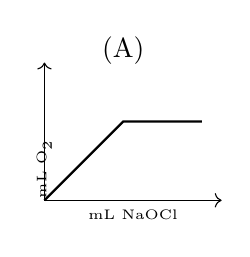
\begin{tikzpicture}[scale=0.5]
\draw[->] (0,0) -- (4.5,0) node[below,pos=0.5] {\tiny mL NaOCl};
\draw[->] (0,0) -- (0,3.5) node[left,rotate=90,pos=0.5] {\tiny mL $\ch{O2}$};
\node at (2,3.8) {(A)};
\draw[thick] (0,0) -- (2,2) -- (4,2);
\end{tikzpicture}
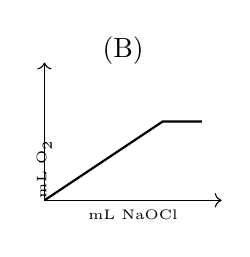
\begin{tikzpicture}[scale=0.5]
\draw[->] (0,0) -- (4.5,0) node[below,pos=0.5] {\tiny mL NaOCl};
\draw[->] (0,0) -- (0,3.5) node[left,rotate=90,pos=0.5] {\tiny mL $\ch{O2}$};
\node at (2,3.8) {(B)};
\draw[thick] (0,0) -- (3,2) -- (4,2);
\end{tikzpicture}

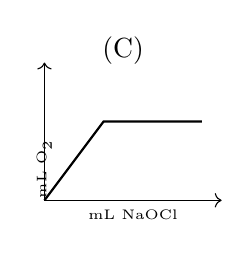
\begin{tikzpicture}[scale=0.5]
\draw[->] (0,0) -- (4.5,0) node[below,pos=0.5] {\tiny mL NaOCl};
\draw[->] (0,0) -- (0,3.5) node[left,rotate=90,pos=0.5] {\tiny mL $\ch{O2}$};
\node at (2,3.8) {(C)};
\draw[thick] (0,0) -- (1.5,2) -- (4,2);
\end{tikzpicture}
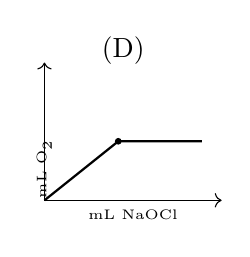
\begin{tikzpicture}[scale=0.5]
\draw[->] (0,0) -- (4.5,0) node[below,pos=0.5] {\tiny mL NaOCl};
\draw[->] (0,0) -- (0,3.5) node[left,rotate=90,pos=0.5] {\tiny mL $\ch{O2}$};
\node at (2,3.8) {(D)};
\draw[thick] (0,0) -- (1.875,1.5) -- (4,1.5);
\filldraw (1.875,1.5) circle (2pt);
\end{tikzpicture}
\end{center}

\item A weighed sample of iron ore is dissolved in 10~mL of 1.0~M hydrochloric acid and then titrated with 0.100~M \ch{KMnO4} to determine the percent iron by mass in the sample. Which glassware is the best choice for measuring the hydrochloric acid?
\begin{enumerate}[label=(\Alph*)]
    \item 50 mL buret \item 10 mL volumetric pipet \item 10 mL graduated pipet \item 10 mL graduated cylinder
\end{enumerate}

\item A 0.1 M aqueous solution containing which metal ion is least intensely colored?
\begin{enumerate}[label=(\Alph*)]
    \item \ch{Cr^{2+}} \item \ch{Mn^{2+}} \item \ch{Co^{2+}} \item \ch{Ni^{2+}}
\end{enumerate}

\item When equal volumes of a 1.0 M ammonium sulfate solution and a saturated solution of barium hydroxide are mixed, what is observed?
\begin{enumerate}[label=\Roman*.]
    \item Gas is evolved.
    \item A white precipitate forms.
\end{enumerate}
\begin{enumerate}[label=(\Alph*)]
    \item I only \item II only \item Both I and II \item Neither I nor II
\end{enumerate}

\item A weighed sample of a copper-nickel alloy is dissolved in a known volume of nitric acid. Which method is most suitable for determining the mass percent of copper in the alloy?
\begin{enumerate}[label=(\Alph*)]
    \item Treatment of an aliquot of the solution with excess iodide, followed by titration of the iodine produced with sodium thiosulfate.
    \item Measurement of the absorbance of the solution at a wavelength of light at which both \ch{Cu^{2+}} and \ch{Ni^{2+}} absorb, and comparison with the absorbances of known standards of the two ions.
    \item Addition of excess sodium hydroxide to the solution, isolation of the metal hydroxides by filtration, and measurement of the mass of the precipitate.
    \item Bubbling hydrogen gas through the solution and measuring the mass of the metal that precipitates from the solution.
\end{enumerate}

\item Which metal ion forms the least soluble perchlorate salt?
\begin{enumerate}[label=(\Alph*)]
    \item \ch{Li+} \item \ch{Mg^{2+}} \item \ch{K+} \item \ch{Ca^{2+}}
\end{enumerate}

\item A sample of malachite, \ch{Cu2CO3(OH)2}, is heated over a Bunsen burner to form \ch{CuO}. The mass percent copper in the sample is calculated based on the mass before and after heating. Which could explain the experimentally determined percent copper being lower than that expected for malachite?
\begin{enumerate}[label=(\Alph*)]
    \item The sample is not heated as strongly as recommended.
    \item The sample is heated more strongly than recommended.
    \item Azurite (\ch{Cu3(CO3)2(OH)2}) is present in the sample.
    \item Goethite (\ch{FeO(OH)}) is present in the sample.
\end{enumerate}

\item A bicycle tire is filled with air to a pressure of 72 psi at a temperature of $25.0^\circ\text{C}$. If the air temperature inside the tire increases to $55.0^\circ\text{C}$ and the volume of the tire increases by 5.0\%, what is the pressure inside the tire?
\begin{enumerate}[label=(\Alph*)]
    \item 69 psi \item 75 psi \item 83 psi \item 166 psi
\end{enumerate}

\item Which \ch{C5H10O} isomer has the highest normal boiling point?
\begin{enumerate}[label=(\Alph*)]
    \item \chemfig{CH_3-CH_2-CH_2-CH_2-CHO}
    \item \chemfig{CH_3-CH_2-CO-CH_2-CH_3}
    \item \chemfig{CH_2=CH-CH(OH)-CH_2-CH_3}
    \item \chemfig{CH_3-C(CH_3)_2-CHO}
\end{enumerate}

\item Two substances Q and R have the same normal boiling point. Substance Q has a larger enthalpy of vaporization than substance R. Which is true about the relative boiling points of the substances at 2.0 atm pressure?
\begin{enumerate}[label=(\Alph*)]
    \item The boiling point of Q is lower than the boiling point of R at 2.0 atm.
    \item The boiling point of Q is higher than the boiling point of R at 2.0 atm.
    \item The boiling points of Q and R are the same at 2.0 atm.
    \item The relative boiling points cannot be predicted from the information given.
\end{enumerate}

\item The density of white tin is $7.28\text{ g cm}^{-3}$ and the density of gray tin is $4.75\text{ g cm}^{-3}$. The conversion of white tin to gray tin, $\ch{Sn}(s, \text{white}) \rightarrow \ch{Sn}(s, \text{gray})$, has a standard enthalpy of reaction of $-2.1\text{ kJ mol}^{-1}$ at 298 K. At 1 atm pressure, white tin and gray tin are in equilibrium at $13^\circ\text{C}$. Which best represents the phase diagram of tin near $13^\circ\text{C}$ and 1 atm?
\begin{enumerate}[label=(\Alph*)]
    \item Gray Sn stable at high T, White Sn stable at low T
    \item White Sn stable at high T, Gray Sn stable at low T with negative slope
    \item Gray Sn stable at low T, White Sn stable at high T with positive slope
    \item White Sn stable at high pressure, Gray Sn stable at low pressure
\end{enumerate}

\item Nickel crystallizes in a face-centered cubic structure. The edge of a unit cell has a length of 352 pm. What is the distance between the nuclei of two adjacent nickel atoms in this lattice?
\begin{enumerate}[label=(\Alph*)]
    \item 117 pm \item 176 pm \item 249 pm \item 305 pm
\end{enumerate}

\item A 10-gram sample of a substance is added to a rigid evacuated 1 L vessel. The pressure in the vessel is measured as a function of temperature. Which graph is obtained if a 10-gram sample of the substance is heated in a 2 L vessel?
\begin{enumerate}[label=(\Alph*)]
    \item A graph with half the slope in the gas phase portion.
    \item A graph with twice the slope.
    \item A graph showing identical phase boundaries.
    \item A graph where condensation occurs at a lower temperature.
\end{enumerate}

\item The phase change $\ch{X}(s) \rightarrow \ch{X}(l)$ has $\Delta G^\circ > 0$ at 300 K. Which statement about this reaction must be correct?
\begin{enumerate}[label=(\Alph*)]
    \item $K_{\text{eq}} < 1$ at 300 K
    \item $\Delta S^\circ < 0$ at 300 K
    \item Liquid X cannot exist at 300 K
    \item The melting point of X is greater than 300 K
\end{enumerate}

\item For which reaction is $\Delta H^\circ_{\text{rxn}}$ closest to $\Delta G^\circ_{\text{rxn}}$?
\begin{enumerate}[label=(\Alph*)]
    \item $2\,\ch{CO2}(g) \rightarrow 2\,\ch{CO}(g) + \ch{O2}(g)$
    \item $2\,\ch{HCl}(g) \rightarrow \ch{H2}(g) + \ch{Cl2}(g)$
    \item $2\,\ch{H2O}(l) \rightarrow 2\,\ch{H2}(g) + \ch{O2}(g)$
    \item $2\,\ch{NaCl}(s) \rightarrow 2\,\ch{Na}(s) + \ch{Cl2}(g)$
\end{enumerate}

\item 2.00 g solid iodine, initially at 300 K, is heated in a sealed vessel maintained at 1.00 atm pressure. The temperature of the sample as a function of the amount of heat added to it is monitored. What is the entropy of vaporization of $\ch{I2}$, $\Delta S^\circ_{\text{vap}}$ at its normal boiling point?
\begin{enumerate}[label=(\Alph*)]
    \item $40.1\text{ J mol}^{-1}\text{K}^{-1}$ \item $52.6\text{ J mol}^{-1}\text{K}^{-1}$ \item $56.8\text{ J mol}^{-1}\text{K}^{-1}$ \item $92.8\text{ J mol}^{-1}\text{K}^{-1}$
\end{enumerate}

\item 20.0 mL of $\ch{NaOH}(aq)$ is titrated against 1.00 M $\ch{HCl}(aq)$ in a well-insulated vessel with constant stirring. Each solution is initially at $22.0^\circ\text{C}$, and the maximum temperature reached is monitored. What is $\Delta H^\circ$ for the reaction that takes place?
\begin{enumerate}[label=(\Alph*)]
    \item $-15\text{ kJ mol}^{-1}$ \item $-31\text{ kJ mol}^{-1}$ \item $-39\text{ kJ mol}^{-1}$ \item $-54\text{ kJ mol}^{-1}$
\end{enumerate}

\item Silver ion reacts with ammonia to form a complex ion:
\[ \ch{Ag+}(aq) + 2\,\ch{NH3}(aq) \rightarrow \ch{Ag(NH3)2+}(aq) \]
In a certain solution at equilibrium at 298 K, $[\ch{Ag+}] = [\ch{NH3}] = [\ch{Ag(NH3)2+}] = C$. What is $\Delta G_{\text{rxn}}$ at 298 K if $[\ch{Ag+}] = [\ch{NH3}] = [\ch{Ag(NH3)2+}] = 0.1C$?
\begin{enumerate}[label=(\Alph*)]
    \item $-5.7\text{ kJ mol}^{-1}$ \item $0\text{ kJ mol}^{-1}$ \item $5.7\text{ kJ mol}^{-1}$ \item $11.4\text{ kJ mol}^{-1}$
\end{enumerate}

\item Equal volumes of 1.00 M $\ch{HSO4-}(aq)$ and 1.00 M $\ch{SO4^{2-}}(aq)$ are mixed. The pH of this solution varies with the reciprocal of the absolute temperature according to the linear equation $y = -1254x + 6.10$. What is the standard enthalpy change for the acid dissociation of $\ch{HSO4-}(aq)$?
\begin{enumerate}[label=(\Alph*)]
    \item $-24.0\text{ kJ mol}^{-1}$ \item $-10.4\text{ kJ mol}^{-1}$ \item $10.4\text{ kJ mol}^{-1}$ \item $24.0\text{ kJ mol}^{-1}$
\end{enumerate}

\item Hydroxide ion reacts with methyl iodide to give methanol in an irreversible second-order reaction with a rate constant $k = 6.5 \times 10^{-5}\text{ L mol}^{-1}\text{s}^{-1}$:
\[ \ch{OH-}(aq) + \ch{CH3I}(aq) \rightarrow \ch{CH3OH}(aq) + \ch{I-}(aq) \]
How long will it take the concentration of $\ch{CH3I}$ to decrease from 0.010 M to 0.0020 M in a 1.00 M solution of sodium hydroxide?
\begin{enumerate}[label=(\Alph*)]
    \item 120 s \item $2.5 \times 10^4\text{ s}$ \item $4.1 \times 10^6\text{ s}$ \item $6.2 \times 10^6\text{ s}$
\end{enumerate}

\item The temperature-dependence of the rate constant of a chemical reaction can be described by the Arrhenius equation, $k = Ae^{-E_a/RT}$. Which elementary chemical reaction has the largest Arrhenius pre-factor $A$?
\begin{enumerate}[label=(\Alph*)]
    \item $\ch{(CH3)3CBr}(aq) \rightarrow \ch{(CH3)3C+}(aq) + \ch{Br-}(aq)$
    \item $\ch{N2O4}(g) \rightarrow 2\,\ch{NO2}(g)$
    \item $\ch{CH3NC}(g) \rightarrow \ch{CH3CN}(g)$
    \item $\ch{(CH3O)2SO2}(aq) + \ch{OH-}(aq) \rightarrow \ch{CH3OH}(aq) + \ch{CH3OSO3-}(aq)$
\end{enumerate}

\item The iodination of acetone is irreversible and has a rate law of $\text{Rate} = k[\ch{CH3COCH3}][\ch{H+}]$:
\[ \ch{CH3COCH3}(aq) + \ch{I3-}(aq) \rightarrow \ch{CH3COCH2I}(aq) + \ch{H+}(aq) + 2\,\ch{I-}(aq) \]
When the reaction is carried out with an initial concentration of $\ch{I3-}$ much smaller than those of either acetone or $\ch{H+}$, the yellow color disappears abruptly at time $t$. How does $t$ depend on the initial concentrations?
\begin{center}
\begin{tabular}{cccc}
 & $[\ch{CH3COCH3}]$ & $[\ch{H+}]$ & $[\ch{I3-}]$ \\ \hline
(A) & Direct & Direct & None \\
(B) & Inverse & Inverse & Direct \\
(C) & Direct & Direct & Inverse \\
(D) & Inverse & Inverse & None \\
\end{tabular}
\end{center}

\item The reaction between A and B is carried out twice, with $[\text{A}]_0 = 0.50\text{ M}$ in each run but with two different initial concentrations of B, resulting in differential exponential decay profiles for B. What can be concluded about the rate law?
\begin{enumerate}[label=(\Alph*)]
    \item $\text{Rate} = (0.0069\text{ s}^{-1})[\text{B}]$
    \item $\text{Rate} = (0.0069\text{ M}^{-1}\text{s}^{-1})[\text{A}][\text{B}]$
    \item $\text{Rate} = (0.014\text{ M}^{-1}\text{s}^{-1})[\text{A}][\text{B}]$
    \item The reaction is first order in B, but the order in A cannot be determined from the available data.
\end{enumerate}

\item Nitrogen dioxide reacts with carbon monoxide with the rate law shown:
\[ \ch{NO2}(g) + \ch{CO}(g) \rightarrow \ch{NO}(g) + \ch{CO2}(g) \quad \text{Rate} = k[\ch{NO2}]^2 \]
Which mechanisms are consistent with this rate law?
\begin{description}
    \item[I.] $2\,\ch{NO2} \rightleftharpoons \ch{N2O4}$ (fast, unfavorable); $\ch{N2O4} + \ch{CO} \rightarrow \ch{N2O3} + \ch{CO2}$ (slow); $\ch{N2O3} \rightarrow \ch{NO} + \ch{NO2}$ (fast)
    \item[II.] $2\,\ch{NO2} \rightarrow \ch{NO} + \ch{NO3}$ (slow); $\ch{NO3} + \ch{CO} \rightarrow \ch{NO2} + \ch{CO2}$ (fast)
\end{description}
\begin{enumerate}[label=(\Alph*)]
    \item I only \item II only \item Both I and II \item Neither I nor II
\end{enumerate}

\item The reaction coordinate diagram of an exothermic reaction that takes place at 300 K shows a standard activation barrier. Which best represents the reaction coordinate diagram for the same reaction at 340 K?
\begin{enumerate}[label=(\Alph*)]
    \item The enthalpy values of reactants, products, and transition state change due to heat capacities, typically slightly flattening or shifting the relative baseline.
    \item The barrier remains structurally similar but effective rate increases.
    \item Enthalpy landscape remains virtually identical as an approximation.
    \item The products become higher in enthalpy than reactants.
\end{enumerate}

\item Pure $\ch{PCl5}$ is placed in a rigid flask so that its pressure at $250^\circ\text{C}$ is 2.000 bar. The gas slowly decomposes to $\ch{PCl3}$ and $\ch{Cl2}$ at this temperature, and the partial pressure of $\ch{Cl2}$ is eventually 0.814 bar. What is the value of $K_p$ for the reaction?
\[ \ch{PCl5}(g) \rightleftharpoons \ch{PCl3}(g) + \ch{Cl2}(g) \]
\begin{enumerate}[label=(\Alph*)]
    \item 0.559 \item 0.686 \item 0.814 \item 1.78
\end{enumerate}

\item What is the maximum concentration of lead(II) ions at equilibrium in a solution with $\text{pH} = 10.50$? The $K_{sp}$ of $\ch{Pb(OH)2}$ is $1.4 \times 10^{-15}$.
\begin{enumerate}[label=(\Alph*)]
    \item $7.1 \times 10^{-6}\text{ M}$ \item $1.4 \times 10^{-8}\text{ M}$ \item $3.5 \times 10^{-9}\text{ M}$ \item $4.4 \times 10^{-12}\text{ M}$
\end{enumerate}

\item The $\text{p}K_a$ of methylammonium ion, $\ch{CH3NH3+}$, is 10.64. What is the percent ionization of a 0.20 M solution of methylamine, $\ch{CH3NH2}$?
\begin{enumerate}[label=(\Alph*)]
    \item 0.0011\% \item 0.071\% \item 1.1\% \item 4.7\%
\end{enumerate}

\item Which statement best describes the differences between a 0.1 M solution of ammonium bicarbonate, $\ch{NH4(HCO3)}$, and a 0.1 M solution of ammonium carbonate, $\ch{(NH4)2CO3}$?
\begin{enumerate}[label=(\Alph*)]
    \item The pH of the ammonium bicarbonate solution is lower because bicarbonate is a weaker base than carbonate.
    \item The pH of the ammonium bicarbonate solution is lower because both ammonium ion and bicarbonate ion can act as Brønsted acids.
    \item The pH of the ammonium bicarbonate solution is higher because it has only half the ammonium ion concentration.
    \item The pH of the ammonium bicarbonate solution is higher because it contains fewer total ions.
\end{enumerate}

\item A mixture of $\ch{N2O4}(g)$ and $\ch{NO2}(g)$ is contained in a vessel whose total volume can change but where the total pressure is maintained at 1.00 atm. The initial temperature is 298 K, and the two gases are in equilibrium:
\[ \ch{N2O4}(g) \rightleftharpoons 2\,\ch{NO2}(g) \quad \Delta H^\circ = 57.6\text{ kJ mol}^{-1} \]
Which changes will result in an increase in the number of moles of $\ch{NO2}$ present at equilibrium?
\begin{enumerate}[label=\Roman*.]
    \item Adding $\ch{Ne}(g)$
    \item Increasing the temperature to 310 K
\end{enumerate}
\begin{enumerate}[label=(\Alph*)]
    \item I only \item II only \item Both I and II \item Neither I nor II
\end{enumerate}

\item Silver iodide is a sparingly soluble salt. Silver also forms a soluble complex ion, $\ch{AgI2-}$, with iodide ion. Which graph of $\log[\ch{Ag}]_{\text{total}}$ vs $\log[\ch{I-}]$ shows a minimum corresponding to the balance between precipitation and complexation?
\begin{enumerate}[label=(\Alph*)]
    \item A linear decrease \item A linear increase \item A parabolic curve opening upwards \item A horizontal line
\end{enumerate}

\item Which species has the largest coefficient when the chemical equation for the disproportionation of white phosphorus in basic solution is balanced?
\[ \_ \ch{P4}(s) + \_ \ch{OH-}(aq) + \_ \ch{H2O}(l) \rightarrow \_ \ch{PH3}(g) + \_ \ch{HPO3^{2-}}(aq) \]
\begin{enumerate}[label=(\Alph*)]
    \item \ch{P4}(s) \item \ch{OH-}(aq) \item \ch{H2O}(l) \item \ch{PH3}(g)
\end{enumerate}

\item Which reagent would spontaneously reduce $\ch{Fe^{2+}}(aq)$ to $\ch{Fe}(s)$ under standard conditions?
\begin{enumerate}[label=(\Alph*)]
    \item \ch{H2}(g) \item \ch{Ni}(s) \item \ch{Sn^{2+}}(aq) \item \ch{Zn}(s)
\end{enumerate}

\item In a test of the selectivity of an electrocatalyst for the reduction of carbon dioxide to methanol, electrolysis is carried out with a constant current of 0.370 A for 155 minutes. Afterwards, the cathodic compartment is found to contain $5.30 \times 10^{-3}$ mol $\ch{CH3OH}$. What is the faradaic yield?
\begin{enumerate}[label=(\Alph*)]
    \item 14.8\% \item 29.7\% \item 59.4\% \item 89.2\%
\end{enumerate}

\item The cathodic compartment of an electrolytic cell is 0.100 M in $\ch{Fe(CN)6^{3-}}$ and $\ch{Cu^{2+}}$. Given $E^\circ(\ch{Fe(CN)6^{3-}}/\ch{Fe(CN)6^{4-}}) = +0.370\text{ V}$ and $E^\circ(\ch{Cu^{2+}}/\ch{Cu}) = +0.337\text{ V}$, which best describes how $\ch{Cu}(s)$ is deposited?
\begin{enumerate}[label=(\Alph*)]
    \item Copper is deposited immediately.
    \item Copper deposition is delayed until $\ch{Fe(CN)6^{3-}}$ is significantly reduced.
    \item Both reduce at identical initial rates.
    \item No copper deposits at all.
\end{enumerate}

\item What is $E^\circ$ for the disproportionation of hydrogen manganate ion in acidic solution?
\[ 5\,\ch{HMnO4-}(aq) + 3\,\ch{H+}(aq) \rightarrow 4\,\ch{MnO4-}(aq) + \ch{Mn^{2+}}(aq) + 4\,\ch{H2O}(l) \]
Given standard reduction potentials: $\ch{MnO4-}/\ch{HMnO4-} = +0.90\text{ V}$ and $\ch{MnO4-}/\ch{Mn^{2+}} = +1.51\text{ V}$.
\begin{enumerate}[label=(\Alph*)]
    \item 0.61 V \item 0.76 V \item 0.99 V \item 1.21 V
\end{enumerate}

\item In the galvanic cell shown, the silver electrode is oxidized to $\ch{Ag+}$ while $\ch{AuCl4-}$ is reduced to elemental Au. The measured cell potential is 0.13 V. Which change will result in the largest value of the measured cell potential?
\begin{center}
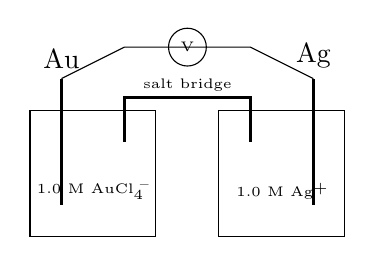
\begin{tikzpicture}[scale=0.8]
\draw (0,0) rectangle (2,2) node[below,pos=0.5] {\tiny 1.0 M $\ch{AuCl4-}$};
\draw (3,0) rectangle (5,2) node[below,pos=0.5] {\tiny 1.0 M $\ch{Ag+}$};
\draw[thick] (0.5,0.5) -- (0.5,2.5) node[above] {Au};
\draw[thick] (4.5,0.5) -- (4.5,2.5) node[above] {Ag};
\draw (0.5,2.5) -- (1.5,3) -- (3.5,3) -- (4.5,2.5);
\draw (2.5,3) circle (0.3) node {\tiny V};
\draw[thick] (1.5,1.5) -- (1.5,2.2) -- (3.5,2.2) -- (3.5,1.5);
\node at (2.5,2.4) {\tiny salt bridge};
\end{tikzpicture}
\end{center}
\begin{enumerate}[label=(\Alph*)]
    \item The concentration of $\ch{AuCl4-}$ is decreased to 0.10 M.
    \item The concentration of $\ch{Cl-}$ is decreased to 0.10 M.
    \item The concentration of $\ch{Ag+}$ is decreased to 0.10 M.
    \item The surface area of the Ag electrode is decreased.
\end{enumerate}

\item One electron in a ground-state gas-phase Ge atom has quantum numbers $(n, l, m_l, m_s)$ of $(4, 1, 1, -\frac{1}{2})$. Which of the following cannot be a valid set of quantum numbers for another electron in this atom?
\begin{enumerate}[label=(\Alph*)]
    \item $(3, 2, 1, \frac{1}{2})$ \item $(4, 0, 0, -\frac{1}{2})$ \item $(4, 1, 0, \frac{1}{2})$ \item $(4, 1, 1, -\frac{1}{2})$
\end{enumerate}

\item How many nodes does the radial wave function of a $3s$ orbital have?
\begin{enumerate}[label=(\Alph*)]
    \item 0 \item 1 \item 2 \item 3
\end{enumerate}

\item Which transition in a gas-phase hydrogen atom would absorb the most energy?
\begin{enumerate}[label=(\Alph*)]
    \item $n=1 \rightarrow n=3$ \item $n=2 \rightarrow n=4$ \item $n=3 \rightarrow n=1$ \item $n=4 \rightarrow n=2$
\end{enumerate}

\item Which element has a gas-phase electron affinity closest to that of sulfur (S)?
\begin{enumerate}[label=(\Alph*)]
    \item O \item P \item Cl \item Se
\end{enumerate}

\item The first ionization energy of gallium ($\text{Ga}, 578.8\text{ kJ mol}^{-1}$) is greater than that of aluminum ($\text{Al}, 577.5\text{ kJ mol}^{-1}$). Which is the best explanation for this?
\begin{enumerate}[label=(\Alph*)]
    \item The $3d$ electrons in gallium imperfectly screen the nuclear charge from the outermost electrons.
    \item The $4p$ orbitals in gallium have an additional radial node.
    \item Gallium has a half-filled subshell.
    \item Higher principal quantum numbers always have lower ionization energies.
\end{enumerate}

\item By what mode does the isotope $\ch{^{31}S}$ undergo radioactive decay?
\begin{enumerate}[label=(\Alph*)]
    \item Alpha decay \item Beta decay \item Gamma decay \item Positron emission
\end{enumerate}

\item Which species has the longest carbon-oxygen bond?
\begin{enumerate}[label=(\Alph*)]
    \item \ch{HCO2-} \item \ch{CO3^{2-}} \item \ch{CO2} \item \ch{COS}
\end{enumerate}

\item Which molecule has a dipole moment of zero?
\begin{enumerate}[label=(\Alph*)]
    \item \ch{BCl3} \item \ch{NI3} \item \ch{AsH3} \item \ch{BrF3}
\end{enumerate}

\item Which ions are linear?
\begin{description}
    \item[I.] \ch{NO2+}
    \item[II.] \ch{ICl2-}
\end{description}
\begin{enumerate}[label=(\Alph*)]
    \item I only \item II only \item Both I and II \item Neither I nor II
\end{enumerate}

\item Which is the best description of the structure of the substance whose empirical formula is \ch{NPF10}?
\begin{enumerate}[label=(\Alph*)]
    \item $\ch{F5N-PF5}$ \item $\ch{F3N-PF7}$ \item $\ch{[NF4+][PF6-]}$ \item $\ch{[PF4+][NF6-]}$
\end{enumerate}

\item Which is the best representation of the three-dimensional arrangement of the atoms in dimethyl carbodiimide, \ch{CH3NCNCH3}?
\begin{enumerate}[label=(\Alph*)]
    \item \chemfig{CH_3-N=C=N-CH_3} (planar trans)
    \item \chemfig{CH_3-N=C=N-CH_3} (orthogonal/allene-like)
    \item \chemfig{CH_3-N=C=N-CH_3} (planar cis)
    \item Linear skeleton
\end{enumerate}

\item Two substances with the formula $\ch{(en)2CoCl3}$ have different aqueous solubilities and different UV-visible spectra. Which is the most likely explanation?
\begin{enumerate}[label=(\Alph*)]
    \item The substances are enantiomers.
    \item The substances are geometric isomers.
    \item One is six-coordinate and the other is seven-coordinate.
    \item One is six-coordinate and the other is four-coordinate.
\end{enumerate}

\item Which molecule is achiral in all of its stereoisomeric forms?
\begin{enumerate}[label=(\Alph*)]
    \item 1,2-cyclohexanediol
    \item 1,3-cyclohexanediol
    \item 1,4-cyclohexanediol
    \item 1,1-cyclohexanediol
\end{enumerate}

\item How many methyl groups are axial in the most stable chair conformation of \textit{trans}-1,2-dimethylcyclohexane?
\begin{enumerate}[label=(\Alph*)]
    \item Zero \item One \item Two \item Three
\end{enumerate}

\item Which series lists the carboxylic acid derivatives in increasing order of reactivity in hydrolysis reactions?
\begin{enumerate}[label=(\Alph*)]
    \item \ch{CH3CH2CONH2} < \ch{CH3CH2COOCH3} < \ch{CH3CH2COCl}
    \item \ch{CH3CH2COOCH3} < \ch{CH3CH2CONH2} < \ch{CH3CH2COCl}
    \item \ch{CH3CH2CONH2} < \ch{CH3CH2COCl} < \ch{CH3CH2COOCH3}
    \item \ch{CH3CH2COOCH3} < \ch{CH3CH2COCl} < \ch{CH3CH2CONH2}
\end{enumerate}

\item Which $\ch{C6H10}$ isomer has the most positive standard enthalpy of formation?
\begin{enumerate}[label=(\Alph*)]
    \item Cyclohexene
    \item 1,3-Hexadiene
    \item Cyclopropene derivative / highly strained ring
    \item 1,5-Hexadiene
\end{enumerate}

\item Which reagent reacts readily with butanal ($\ch{CH3CH2CH2CHO}$), but not with 2-pentanone ($\ch{CH3CH2CH2COCH3}$)?
\begin{enumerate}[label=(\Alph*)]
    \item $\ch{K2Cr2O7}$ in aqueous $\ch{H2SO4}$
    \item $\ch{I2}$ in aqueous $\ch{NaOH}$
    \item $\ch{CH3MgBr}$ in $\ch{Et2O}$
    \item $\ch{NaBH4}$ in $\ch{CH3OH}$
\end{enumerate}

\item $\alpha$-D-glucose and $\beta$-D-glucose interconvert in aqueous solution at pH 7 (mutarotation). Which best describes the intermediate in this isomerization?
\begin{enumerate}[label=(\Alph*)]
    \item A planar oxacyclohexane
    \item An acyclic aldohexose
    \item A disaccharide
    \item An achiral glycoside
\end{enumerate}

\end{enumerate}

\end{document}